% !TEX root=report.tex
\section{Evaluation} \label{sec:evaluation}

The CouchSurfing dataset was made available to the authors in the form of an anonymized MySQL database dump.

Due to the communicated need of CouchSurfing developers, we focused our evaluation on the host perspective, where accuracy in predicting rejects is not as important as accuracy in predicting a successful visitor, and assistance is particularly important when the host faces a lot of couch requests at once.
Therefore, we look at all competitor sets that have a winner, grouped by cardinality.

We compare our system against a random baseline as well as several rule-based approaches that may form the system currently deployed at Couchsurfing.
These baselines present simple feature-based rules, such as ordering by the number of references or friends.
We call these single-feature baselines.
Although the exact ranking model currently deployed at CouchSurfing was not shared with us, we were told that it is a simple rule-based approach that most likely involves the parameters mentioned above.

The specific baselines were:
\begin{itemize}
\item \textit{Random} Baseline that predicts a random element from the
competitor set
\item \textit{Priority1/2} Baseline that CouchSurfing presumably uses
to rank surfers and hosts on their website
\item \textit{Vouched} The number of people that vouched for a given user
\item \textit{References/to} References given to and received from other users
\item \textit{Friend links} Number of friends on CouchSurfing
\end{itemize}

We use two different measures to evaluate performance: Prediction Accuracy (PA), and Average Normalized Winner Rank (ANWR).
Prediction Accuracy is the fraction of correctly predicted winners from several competitor sets.
Average Normalized Winner Rank is a more general measure that captures what position the actual winner has in the computed ranking.
We normalize the rank to be on $[0,1]$.
Note that a prediction only counts as a positive towards PA if it occured at the first place in the ranking.
The ANWR is a less strict evaluation metric in this case, but it may better represent the actual use case we are developing for.

We compute these two measure on the CouchSurfing Data that has 11 million couch request, grouped into 5.5 million competitor sets.
We split these competitor sets into a training, validation, and test set (at a 60/20/20\% split).
To ensure that we do not look ahead into the future to make predictions easier, we split the data chronologically.

Note that the state of the system at the time of feature computation lies ``in the future'' relative to the request being represented.
This has certain effects, described below.

\begin{figure}[ht]
\centering
\subfloat[Prediction Accuracy (higher is better)]{
  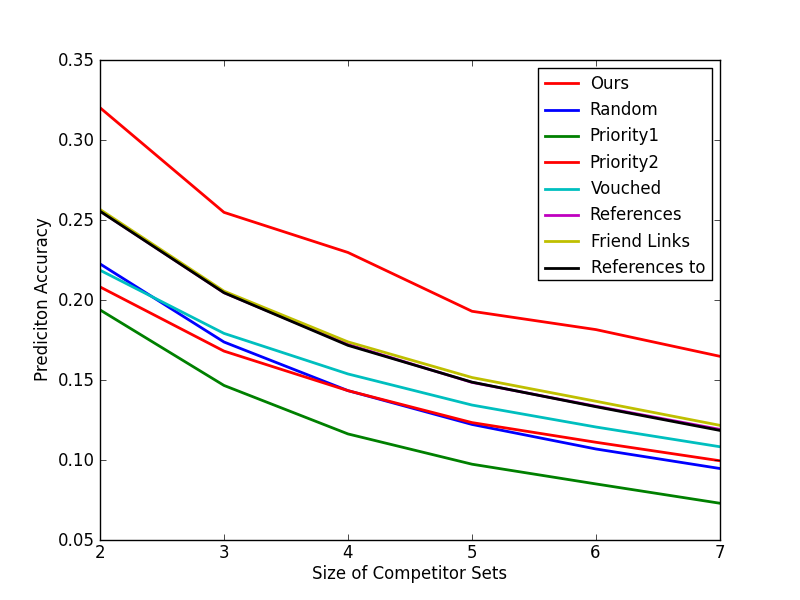
\includegraphics[width=0.75\linewidth]{figures/prediciton_accuracy.png}
}\\
\subfloat[Average Winner Rank (lower is better)]{
  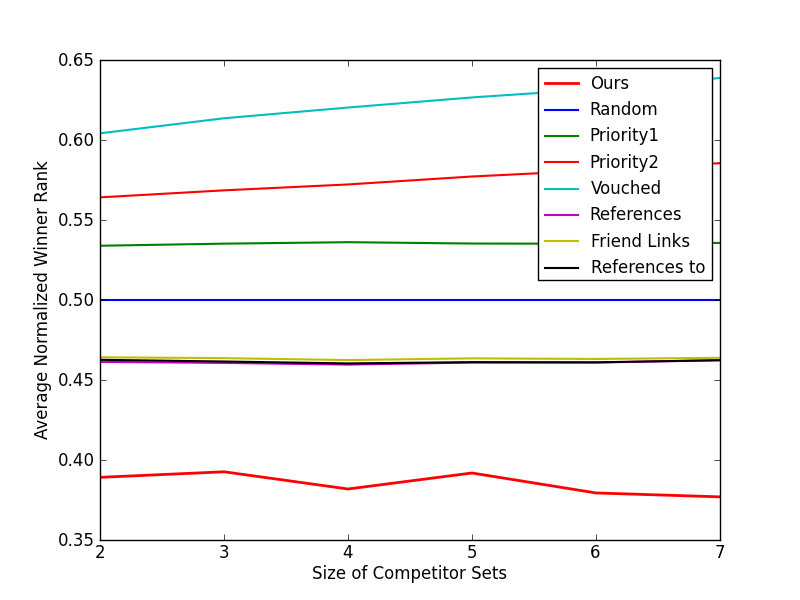
\includegraphics[width=0.75\linewidth]{figures/avg_winner_rank.png}
}
\caption{Our evaluations: prediction accuracy and average winner rank. In both cases, we do better than all baselines.}
\label{fig:eval}
\end{figure}

For a summary of the results see \autoref{fig:eval} which shows PA and ANWR on competitor sets of a certain minimum cardinality.
One can observe that we consistently outperform the baselines by several percent.
For larger competitor sets, the recommendation or ranking task becomes harder and performance drops.
Especially in this regime, our algorithm supports hosts better in choosing the right couch surfer to accept.

Due to the normalization the ANWR error metric stays roughly constant as cardinality of the set increases.
The average rank for the random baseline is 0.5 (``the middle'').
Interestingly, some of the single-feature baselines do worse than the random baseline (e.g. the number of people that have vouched to you).
The number of friends and the number of references performs better than random.
Using our system, on average, a host needs to browse 39\% of the list compared to 46\% for the the second best approach.

\subsection{Discussion}
Why is this such a hard problem? First of all, notice that estimating probabilities including the possibility of rejection is much harder than just ranking of candidates due to the fact that rejectance might have nothing to do with the candidates themself or the hosts preference but may simply be dependent on the host's availability. This availability is hard to to infer automatically from the user's profile. For us it was impossible to capture this kind of time-dependent information because we were only supplied with the current state of the CouchSurfing database.

Furthermore, note that this also means that we cannot know e.g. when two users became friends on the network. This can lead to interfering behavior. Assume that we know that host $h$ accepted surfer $s$ from  a competitor set $S$ and we know that they are friends. Our model infers that it this friendship might be \textit{the} critical and discriminative feature. However, $h$ and $s$ might not have been friends before the accepted couchrequest but only after they spent some time with each other. Similarly, our current model does not capture other temporal relationships such as whether host and surfer had been in contact before the actual request. We hypothesize that accurate modeling of this temporal structure in the data should improve performance significantly.
